\chapter{Análisis}

\section{Análisis de requisitos}

\subsection{Requisitos no funcionales}

\begin{table}[H]
	\begin{center}
		\begin{tabular}{|p{1.5cm}| p{10.5cm}|}
			\hline
			Código & Descripción \\
			\hline
			RNF-1  & La aplicación tratara de un simulador. Dicha simulación se realizara sobre mapas online\\ \hline
			RNF-2  & La navegación por los menús de la aplicación se realizara mediante una interfaz gráfica\\ \hline
			RNF-3  & Los textos por defecto de la aplicación serán en inglés\\ \hline
			RNF-4  & La autenfiticación de usuarios se realizará mediante web tokens\\ \hline
			RNF-5  & La interfaz gráfica debe ser responsive desarrollada con bootstrap\\ \hline
			RNF-6  & El back-end debe ser desarrollado con node.js, sockets.io y express \\ \hline
			RNF-7  & El front-end debe ser desarrollado con Angular.js\\ \hline
		\end{tabular}
		\caption{Requisitos no funcionales}
		\label{tabla:requisitosNoFuncionales2}
	\end{center}
\end{table}

\newpage

\subsection{Requisitos funcionales}


\begin{longtable}[H]{|c|p{10cm}|}
	% aquí añadimos el encabezado de la primera hoja.
	\hline
	Código & Descripción \\
	\hline \hline
	\endfirsthead
	
	% aquí añadimos el encabezado del resto de hojas.
	\hline
	Código & Descripción \\
	\hline \hline
	\endhead
	
	% aquí añadimos el fondo de todas las hojas, excepto de la última.
	\multicolumn{2}{c}{}
	\endfoot
	
	% aquí añadimos el fondo de la última hoja.
	\endlastfoot
	
	% aquí añadimos el cuerpo de la tabla.
	RF-1  & La aplicación permitirá crear un nuevo usuario\\ \hline
	RF-2  & La aplicación permitirá al usuario buscar mapas por su nombre, tipo, estado, cuidad y fecha de creación\\ \hline
	RF-3  & La aplicación permitirá al usuario crear un nuevo mapa\\ \hline
	RF-4  & La aplicación permitirá al usuario crear una nueva escena asociada a un mapa existente\\ \hline
	RF-5  & La aplicación listara todas las escenas de un mapa\\ \hline
	RF-6  & La aplicación permitirá al usuario editar un mapa existente\\ \hline
	RF-7  & La aplicación permitirá al usuario editar las escenas de un mapa existente\\ \hline
	RF-8  & La aplicación permitirá al usuario crear un nuevo tipo de objeto estático\\ \hline
	RF-9  & La aplicación permitirá al usuario crear un nuevo tipo de objeto dinámico\\ \hline
	RF-10 & La aplicación listará todos los tipos de objetos estáticos creados\\ \hline
	RF-11 & La aplicación listará todos los tipos de objetos dinámicos creados\\ \hline
	RF-12 & La aplicación permitirá al usuario editar los objetos estáticos credos\\ \hline
	RF-13 & La aplicación permitirá al usuario editar los objetos dinámicos creados\\ \hline
	RF-14 & La aplicación permitirá al usuario cambiar el nombre\\ \hline
	RF-15 & La aplicación permitirá al usuario cambiar su contraseña\\ \hline
	RF-16 & La aplicación permitirá al usuario cambiar la imagen asociada a un usuario\\ \hline
	RF-17 & La aplicación permitirá al usuario configurar un nuevo tipo de recomendador\\ \hline
	RF-18 & La aplicación permitirá al usuario editar la configuración de recomendador existente\\ \hline
	RF-18 & La aplicación permitirá al usuario asociar un recomendador existente a una escena\\ \hline
	RF-19 & La aplicación permitirá al usuario definir los límites de una escena\\ \hline
	RF-20 & La aplicación permitirá al usuario asociar un objeto estático a una escena\\ \hline
	RF-21 & La aplicación permitirá al usuario cargar todos los objetos estáticos desde un fichero JSON\\ \hline
	RF-22 & La aplicación permitirá asociar un objeto dinámico y su definir su ruta en una escena\\ \hline
	RF-23 & La aplicación permitirá al usuario cargar todos los objetos dinámicos y sus rutas desde un fichero JSON\\ \hline
	RF-24 & La aplicación listará todos objetos estáticos asociados a una escena \\ \hline
	RF-25 & La aplicación listará todos los objetos dinámicos asociados a una escena \\ \hline
	RF-26 & La aplicación permitirá borrar un objeto estático asociado a una escena\\ \hline
	RF-27 & La aplicación permitirá borrar un objeto dinámico asociado a una escena\\ \hline
	RF-28 & La aplicación permitirá al usuario elegir un si mapa es colaborativo o no\\ \hline
	RF-29 & La aplicación permitirá al usuario ejecuta una simulación sobre la escena de un mapa\\ \hline
	RF-30 & La aplicación permitirá al usuario solicitar recomendaciones mientras se está ejecutando una simulación siempre y cuando el recomendador asociado a la escena es de tipo pull\\ \hline
	RF-31 & El usuario recibirá recomendaciones sin haberlas solicitado siempre y cuando el recomendador asociado a la escena de es tipo push\\ \hline
	RF-32 & El usuario puede arrancar/pausar una simulación\\ \hline
	RF-33 & La aplicación permitirá al usuario generar de forma aleatoria los grafos de movimiento de los vehículos \\ \hline	
	\caption{Requisitos funcionales}
	\label{tabla:requisitosFuncionales2}
\end{longtable}


\section{Objetivos de Usabilidad}

La Usabilidad, según el estándar ISO 9241-11, se define como la medida en la que un producto se puede usar por determinados usuarios para conseguir objetivos específicos de efectividad, eficiencia y satisfacción de un contexto de uso específico.  

Así que para poder garantizar la calidad y la satisfacción de los usuarios tenemos que tener en cuenta los objetivos de usabilidad descritos:  

\begin{itemize}
	\item {\bfseries Efectividad}: asegurar que la aplicación desempeñe correctamente todos los objetivos de la aplicación.  	
	\item {\bfseries Eficiencia}: asegurar que cada objetivo de aplicación sea realizado en el menor tiempo posible desempeñando correctamente su tareas .
	\item {\bfseries Utilidad}:para que el sistema pueda hacer todas las tareas que el usuario deba hacer, la aplicación tendrá conexión a Internet ya que establecerá conexión con un servidor en el que se encuentra toda la información de los productos. Siempre y cuando la conexión sea satisfactoria, el usuario podrá realizar las tareas descritas en el apartado de análisis de requisitos funcionales. 
	\item {\bfseries Seguridad}: asegurar que la aplicación evite situaciones de pérdida de información, evitar que se cuelgue y garantizar la confidencialidad de la información ya que la aplicación tiene acceso a Internet.
\end{itemize}	 

\begin{longtable}[H]{|p{3cm}|p{3cm}|p{3cm}|p{3cm}|}
	% aquí añadimos el encabezado de la primera hoja.
	\hline
	Objetivos & Eficacia & Eficiencia  & Satisfacción \\
	\hline \hline
	\endfirsthead
	
	% aquí añadimos el encabezado del resto de hojas.
	\hline
	Objetivos  & Eficacia & Eficiencia  & Satisfacción \\
	\hline \hline
	\endhead
	
	% aquí añadimos el fondo de todas las hojas, excepto de la última.
	\multicolumn{2}{c}{}
	\endfoot
	
	% aquí añadimos el fondo de la última hoja.
	\endlastfoot
	
	% aquí añadimos el cuerpo de la tabla.
			Utilizabilidad global  & Usuarios que terminan la tarea con éxito: 99\% de usuarios  & Tiempo de realización de tareas:8 seg.  & Frecuencia de quejas: 2 - 4 de cada 100 \\ \hline
			
			Satisface las necesidades de los usuarios habituales  & Tareas terminadas con éxito: 95\% de tareas  & Tiempo de realización de tareas: 5 seg. & Evaluación de satisfacción en el uso de las funciones: 9/10\\ \hline
			
			Satisface las necesidades de los usuarios noveles   & Tareas terminadas con éxito en el primer intento: 90\% de tareas  & Tiempo de realización de las tareas: 15 seg. & Tiempo de uso no obligatorio: 10 seg. - 20 seg. \\ \hline
			
			Facilidad de aprendizaje  & Número de funciones aprendidas: 100\% de las funciones  & Número de usos para aprendizaje: 2 - 3 usos  & Evaluación de la facilidad de aprendizaje: 8/10 \\ \hline
			
			Tolerancia a errores  & Errores registrados o corregidos por el sistema: 100\% de errores & Tiempo empleado en corregir errores: 30 seg. & tratamiento de errores: 9/10 \\ \hline
			
			Legibilidad  & Palabras leídas correctamente a distancia normal: 100\% de palabras  & Tiempo necesarios par leer la pantalla: 10 seg. - 15 seg.  & Evaluación de las molestias visuales: 1/10 (menos nota implica menor molestia)  \\ \hline
	
	\caption{Objetivos de usabilidad}
	\label{tabla:objetivosUsabilidad}
\end{longtable}

\newpage

\section{Diagrama de casos de uso}

En esta sección se mostrará el diagrama de casos de usos analizado. El diagrama de casos de uso se ha divido en dos partes porque es demasiado grande para ser visualizado correctamente en una solo imagen.

\begin{figure}[H]
	\centering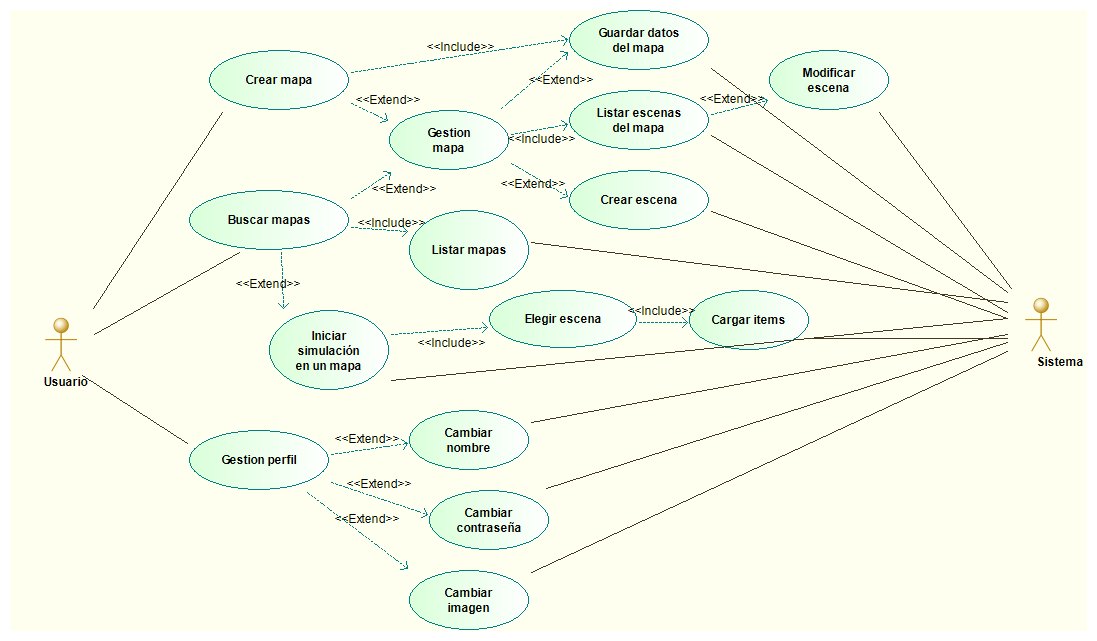
\includegraphics[scale=0.35]{imagenes/casos-de-uso-1.png}
	\caption{Diagrama de casos de uso parte 1}
	\label{img:casosDeUso1}
\end{figure}

\begin{figure}[H]
	\centering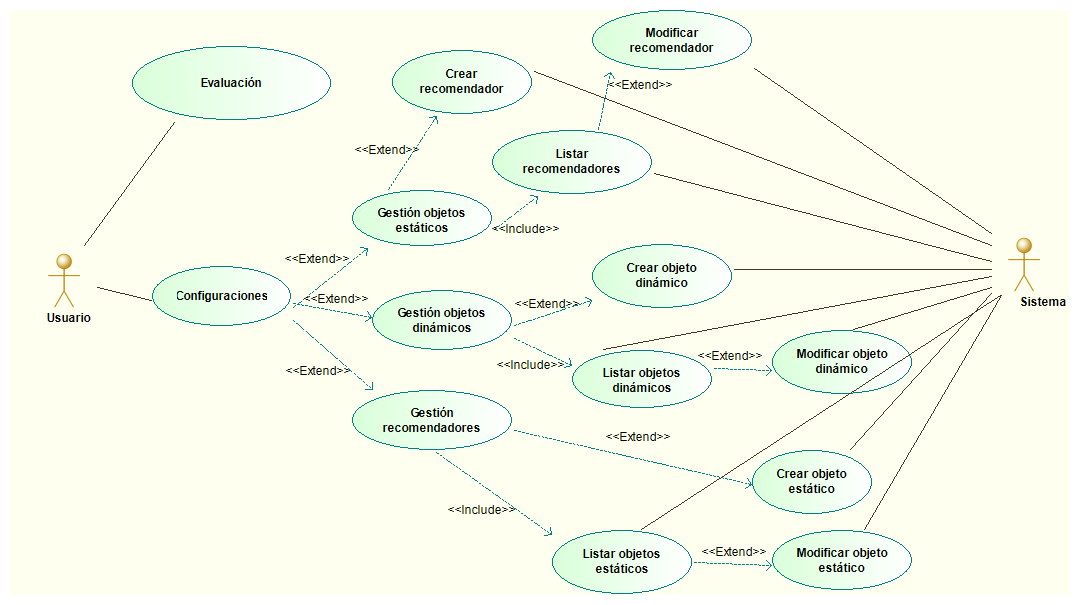
\includegraphics[scale=0.35]{imagenes/casos-de-uso-2.png}
	\caption{Diagrama de casos de uso parte 2}
	\label{img:casosDeUso2}
\end{figure}
